\documentclass[12pt,aspectratio=169]{beamer}
\usetheme{metropolis}
\setbeamersize{text margin left=.5cm,text margin right=.5cm}
\usepackage[lf]{carlito}
\usepackage{siunitx}
\usepackage{tikz}
\usepackage{mathpazo}
\usepackage{bm}
\usepackage{mathtools}
\usepackage[ISO]{diffcoeff}
\diffdef{}{ op-symbol=\mathsf{d} }
\usepackage{xcolor,colortbl}

\setmonofont{Ubuntu Mono}
\setlength{\parskip}{0pt}
\renewcommand{\baselinestretch}{1}

\sisetup{
  inter-unit-product=\cdot,
  per-mode=symbol
}

\tikzset{
  >=latex
}

%\newcommand{\iii}{\hat{\bm\imath}}
%\newcommand{\jjj}{\hat{\bm\jmath}}
%\newcommand{\kkk}{\hat{\bm k}}


\title{Class 17: Magnetism, Part 1}
\subtitle{Advanced Placement Physics C}
\author[TML]{Dr.\ Timothy Leung}
\institute{Olympiads School}
\date{Updated: Summer 2022}

\newcommand{\pic}[2]{
  \includegraphics[width=#1\textwidth]{#2}
}
\newcommand{\eq}[2]{
  \vspace{#1}{\Large
    \begin{displaymath}
      #2
    \end{displaymath}
  }
}
%\newcommand{\iii}{\ensuremath\hat{\bm{\imath}}}
%\newcommand{\jjj}{\ensuremath\hat{\bm{\jmath}}}
%\newcommand{\kkk}{\ensuremath\hat{\bm{k}}}
\newcommand{\iii}{\ensuremath\hat\imath}
\newcommand{\jjj}{\ensuremath\hat\jmath}
\newcommand{\kkk}{\ensuremath\hat k}


\begin{document}

\begin{frame}
  \maketitle
\end{frame}


\section{Magnetic Field}

\begin{frame}{Review of Magnetic Field}
  \begin{itemize}
  \item Magnetism is generated by moving charged particles, e.g.\ a single
    charge, or an electric current
  \item It can also be generated by permanent magnets, or Earth
  \end{itemize}
\end{frame}



\begin{frame}{Review of Magnetic Field}
  \begin{itemize}
  \item Magnetism affects other \emph{moving} charged particles
  \item The vector field is called the \textbf{magnetic field}
  \item Magnetic field has unit \textbf{tesla}
  \item Magnetic field lines have no ends---they always run in a loop
  \end{itemize}
\end{frame}



\begin{frame}{Magnetic Field Generated by a Moving Point Charge}
  \begin{center}
    \pic{.35}{pointchargeB}
  \end{center}
  A point charge generates an electric field $\vec E$. When it's moving, it
  also generates a magnetic field $\vec B$, given by the equation:

  \eq{-.1in}{
    \boxed{\vec B=\frac{\mu_0}{4\pi}\frac{q\vec v\times\hat r}{r^2}}
  }

  The direction of $\vec B$ can be obtained by applying the
  \emph{right-hand rule} if you are not confident with cross products.
\end{frame}



\begin{frame}{Reminder on the cross product}
  Whenever the ``right-hand rule'' is mentioned, or when an equation has
  ``$\sin\theta$'' in it, that usually means that the equation involces a
  cross product in it. Just a reminder on a few properties:
  \begin{itemize}
  \item If $\vec C=\vec A\times\vec B$, then $\vec C$ is perpendicular to both
    $\vec A$ and $\vec B$.
  \item The length of the cross product of two vectors is:
    
    \eq{-.1in}{
      |\vec A\times\vec B|=|\vec A||\vec B|\sin\theta
    }
    where $\theta$ is the angle between $\vec A$ and $\vec B$
  \item Cross products are anti-commutable:

    \eq{-.1in}{
      \vec A\times\vec B=-\vec B\times\vec A
    }
  \end{itemize}
\end{frame}



\begin{frame}{Magnetic Field Generated by a Moving Point Charge}

  \eq{0in}{
    \boxed{\vec B=\frac{\mu_0}{4\pi}\frac{q\vec v\times\hat r}{r^2}}
  }
  \begin{center}
    \begin{tabular}{l|c|c}
      \rowcolor{pink}
      \textbf{Quantity} & \textbf{Symbol} & \textbf{SI Unit} \\ \hline
      Magnetic field                  & $\vec B$ & \si\tesla \\
      Charge                          & $q$      & \si\coulomb \\
      Velocity of the charge          & $\vec v$ & \si{\meter\per\second}\\
      Distance from the moving charge & $r$      & \si\metre\\
      Radial outward unit vector from the charge & $\hat r$ & no units\\
      Permeability of free space & $\mu_0$ & \si{\tesla\metre\per\ampere}
    \end{tabular}
  \end{center}
  \textbf{Permeability of free space} (or \textbf{vacuum permeability}) is a
  constant with a value of
  $\mu_0=4\pi\times\num{e-7}\;\si{\tesla\metre\per\ampere}$. It measures how
  well a space can become magnetized.
\end{frame}



\begin{frame}{Biot-Savart Law}
  \begin{columns}
    \column{.25\textwidth}
    \pic1{bsav}
    
    \column{.75\textwidth}
    An electric current is really many charges particles moving along a wire;
    each charge creating its own magnetic field.
    The total magnetic field in the wire is the integral of the contribution
    ($\dl{\vec B}$) of the current ($I$) from each infinitesimal sections
    ($\dl{\vec L}$) of the wire, given by the \textbf{Biot-Savart law}:
  
    \eq{-.1in}{
      \boxed{
        \dl{\vec B}=\frac{\mu_0}{4\pi}\frac{I\dl{\vec L}\times\hat r}{r^2}
      }
    }

    The magnetic field in the diagram goes \emph{into} the page
  \end{columns}
\end{frame}



\begin{frame}{Magnetic Field Generated By an Infinitely Long Wire}
  \begin{columns}
    \column{.2\textwidth}
    \pic1{magcur2}
    
    \column{.7\textwidth}
    Integrating Biot-Savart law for a point at radial distance $r$ from an
    \emph{infinitely-long wire} gives a simple expression:

    \eq{-.1in}{
      \boxed{\vec B=\frac{\mu_0(\vec I\times\hat r)}{2\pi r}}
      \quad\text{or}\quad
      \boxed{B=\frac{\mu_0I}{2\pi r}}
    }

    The magnitude and direction current ``vector'' $\vec I$ is
    straightforward
    \begin{tabular}{l|c|c}
      \rowcolor{pink}
      \textbf{Quantity} & \textbf{Symbol} & \textbf{SI Unit} \\ \hline
      Magnetic field      & $\vec B$ & \si\tesla \\
      Current             & $\vec I$ & \si\ampere \\
      Radial direction from the wire & $\hat r$ & (no units)\\
      Radial distance from the wire  & $r$      & \si\metre
    \end{tabular}
  \end{columns}
\end{frame}


\begin{frame}{Current-Carrying Wire Loop}
  \begin{columns}
    \column{.35\textwidth}
    \pic1{curloo}

    \column{.65\textwidth}
    When we shape the current-carrying wire into a loop, we can (again) use
    the Biot-Savart law to find the magnetic field away from it.

    \vspace{.2in}
    One loop isn't very interesting (except when you're integrating Biot-Savart
    law) but what if we have many loops
  \end{columns}
\end{frame}



\begin{frame}{Wounding Wires Into a Coil}
  \begin{itemize}
  \item A \textbf{solenoid} is when you wound a wire into a coil
  \item You create a magnet very similar to a bar magnet, with an effective
    north pole and a south pole
  \item Magnetic field inside the solenoid is uniform
  \item Magnetic field strength can be increased by the addition of an iron core
  \end{itemize}
  \begin{center}
    \pic{.5}{barsol}
  \end{center}
\end{frame}



\begin{frame}{A Practical Solenoid}
  A practical solenoid usually has hundreds or thousands of turns:
  \begin{center}
    \pic{.45}{1020201515330450255}
  \end{center}

  \vspace{-.2in}
  This ``air core'' coil is used for high school and university experiments. It
  has approximately 600 turns of copper wire wound around a plastic core.
\end{frame}



\begin{frame}{Magnetic Field Inside a Solenoid}
  \begin{columns}
    \column{.3\textwidth}
    \pic1{magneticfield4}
    
    \column{.7\textwidth}
    The magnetic field \textbf{inside} a solenoid is uniform, with its strength
    given by:
    
    \eq{-.1in}{
      \boxed{B=\frac{\mu NI}{\ell}}
    }
    
    Direction of $\vec B$ determined by \textbf{right-hand rule}
    \begin{center}
      \begin{tabular}{l|c|c}
        \rowcolor{pink}
        \textbf{Quantity} & \textbf{Symbol} & \textbf{SI Unit} \\ \hline
        Magnetic field intensity & $B$    & \si\tesla \\
        Number of coils          & $N$    & \\
        Length of the solenoid   & $\ell$ & \si\metre \\
        Current                  & $I$    & \si\ampere \\
        Effective permeability   & $\mu$  & \si{\tesla.\metre\per\ampere}
      \end{tabular}
    \end{center}
  \end{columns}
\end{frame}


\section{Permanent Magnets}

\begin{frame}{Permanent Magnets}
  Permanent magnets is also based on the motion of charges. This is the
  ``non-technical'' version\ldots

  \begin{enumerate}
  \item Electrons inside an atom \emph{spin}. A spinning electron therefore has
    an angular momentum, and generates its own tiny magnetic field.
    \begin{center}
      \pic{.3}{Electron-spin}
    \end{center}
    However, in most full ``shells'', the spin of these electrons are paired,
    so the magnetic fields cancel each other.
  \end{enumerate}
\end{frame}




\begin{frame}{Permanent Magnets}
  \begin{enumerate}
    \setcounter{enumi}{1}
  \item The orbits of electrons are not always filled, therefore some atoms do
    create some (very small) magnetic field.
    \begin{center}
      \pic{.4}{paramagnetic}
    \end{center}
    The atoms that have unpaired electrons are called \textbf{paramagnetic}
    because they are attracted to magnets; atoms that have no unpaired
    electrons are called \textbf{diamagnetic}.
  \end{enumerate}
\end{frame}



\begin{frame}{Permanent Magnets}
  \begin{enumerate}
    \setcounter{enumi}{2}
  \item While many atoms exhibit paramagnetism, they do not make good magnets,
    because the atoms are most often arranged in a way where the magnetic fields
    cancel. This is callled \textbf{ferrimagnetism}:
    \begin{center}
      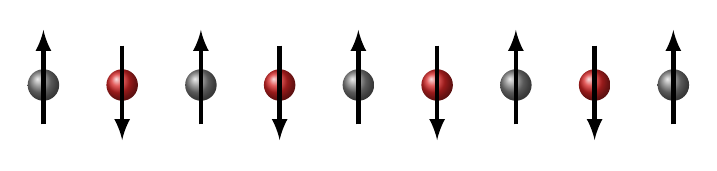
\begin{tikzpicture}
        \foreach\x in {0,2,...,8}{
          \shade[ball color=gray] (\x,0) circle (.2);
          \draw[ultra thick,->] (\x,-.5)--(\x,.7);
        }
        \foreach\x in {1,3,5,7}{
          \shade[ball color=red!70!gray] (\x,0) circle (.2);
          \draw[ultra thick,->] (\x,.5)--(\x,-.7);
        }
        
      \end{tikzpicture}\\
      Ferrimagnetic
    \end{center}
    When they do not cancel, then they can become magnets. This is called
    \textbf{ferromagnetism}:
    \begin{center}
      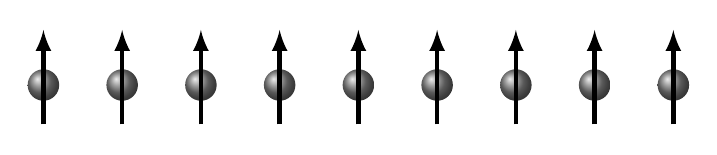
\begin{tikzpicture}
        \foreach\x in {0,1,...,8}{
          \shade[ball color=gray] (\x,0) circle (.2);% node[below right]{$m$};
          \draw[ultra thick,->] (\x,-.5)--(\x,.7);
        }
      \end{tikzpicture}\\
      Ferromagnetic
    \end{center}
    Transitional elements such as iron, nickel and cobalt, and their alloys
    will exhibit ferromagnetism.
  \end{enumerate}
\end{frame}



\begin{frame}{Permanent Magnets}
  \begin{enumerate}
    \setcounter{enumi}{3}
  \item The atoms in these ferromagnetic materials are arranged in ``domains''
    wher their magnetic moment is aligned. In the presence of a strong
    external magnetic field, these domains will line up, creating a magnet.
    \begin{center}
      \pic{.6}{domain}
    \end{center}
  \end{enumerate}
\end{frame}


    
\begin{frame}{Earth}
  Earth is also a ``permanent'' magnet, with the \emph{magnetic south pole}
  located near the geographic north pole, and the \emph{magnetic north pole}
  located near the geographic south pole. The poles are tilted by
  $\approx\ang{11}$ from the spin axis.
  \begin{center}
    \pic{.5}{mearthbar}
  \end{center}
  The exact nature of Earth's magnetic field is not known, although it may be
  related to ``generator effect'' from Earth's rotation, circulating the
  outer-core fluid around.
\end{frame}



\section{Amp\`{e}re's Law}

\begin{frame}{Amp\`{e}re's Law}
  \begin{columns}
    \column{.25\textwidth}
    \pic1{amlaw}
    
    \column{.75\textwidth}
    Like Gauss's law is used to calculate electric fields,
    \textbf{Amp\`{e}re's law} is used to calculate the magnetic field for
    symmetric configurations:

    \eq{-.1in}{
      \boxed{\oint_C \vec B\cdot\dl{\vec\ell}=\mu_0 I_C}
    }
    where
    \begin{itemize}
    \item $C$ is a closed curve around a current (``Amperian loop'')
    \item $\dl{\vec\ell}$ is an infinitesimal length along the closed curve
    \item $I_c$ is the net current that penetrates the area bounded by $C$
    \end{itemize}
  \end{columns}
\end{frame}



\begin{frame}{Application of Amp\`{e}re's Law: Infinitely Long Wire}
  \begin{columns}
    \column{.3\textwidth}
    \pic1{4iM3O}

    \column{.7\textwidth}
    An \emph{infinitely} long wire must generate a magnetic field that only
    depend on radial distance. We place an Amperian loop as a circle of radius
    $r$ inside the toroid. Amp\`{e}re's law reduces to:

    \eq{-.1in}{
      \oint_C \vec B\cdot\dl{\vec\ell}=\mu_0 I_C
      \;\rightarrow\;
      B(2\pi r)=\mu_0 I
    }
      
    From this, we get our expression of the magnetic field from an infinitely
    long wire:
      
    \eq{-.1in}{
      B=\frac{\mu_0 I}{2\pi r}
    }
  \end{columns}
\end{frame}



\begin{frame}{Toroid}
  \begin{columns}
    \column{.3\textwidth}
    \pic1{toroid}

    {\scriptsize A toroid consists of a current-\\
      carrying wire wound around a donut-shaped core \par}
    
    \column{.7\textwidth}
    Another application of Amp\`{e}re's law is the \textbf{toroid}. This time,
    we put our loop at $a<r<b$ inside the toroid. Once again, because of
    symmetry, Amp\`{e}re's law reduces to:

    \vspace{-.3in}{\large
      \begin{align*}
        \oint_C \vec B\cdot\dl{\vec\ell} &=\mu_0 I_C\\
        B(2\pi r)&=\mu_0 NI\\
        B&=\frac{\mu_0 NI}{2\pi r}
      \end{align*}
    }

    where $N$ is the number of times the wire is wound around the core
  \end{columns}
\end{frame}


\begin{frame}{Toroid}
  \begin{columns}
    \column{.3\textwidth}
    \pic1{toroid}

    \column{.7\textwidth}
    When the loop is placed at $r<a$, there is no enclosed
    current, and therefore the magnetic field is zero:

    \eq{-.1in}{
      B=0\quad\text{for}\quad r<a
    }

    \vspace{-.2in}When the loop is placed at $r>b$, the amount of current
    penetrating the loop is the same in both direction, i.e.\ $I_c=0$, and

    \eq{-.1in}{
      B=0\quad\text{for}\quad r>b
    }
    
    \vspace{-.1in}In fact, magnetic field \emph{only} exists inside the core,
    between $a$ and $b$.
  \end{columns}
\end{frame}




\section{Magnetic Force}

\begin{frame}{So What Does the Magnetic Field Do?}{In Classical Physics}
  \begin{columns}
    \column[t]{.3\textwidth}
    \begin{center}
      Gravitational Field $\vec g$
    \end{center}
    \begin{itemize}
    \item Generated by massive objects
    \item Affects massive objects
    \end{itemize}

    \column[t]{.3\textwidth}
    \begin{center}
      Electric Field $\vec E$
    \end{center}
    \begin{itemize}
    \item Generated by charged particles
    \item Affects charged particles
    \end{itemize}

    \column[t]{.4\textwidth}
    \begin{center}
      Magnetic Field $\vec B$
    \end{center}
    \begin{itemize}
    \item Generated by \emph{moving} charged particles
    \item Affects moving charged particles
    \end{itemize}
  \end{columns}
\end{frame}



\begin{frame}{Lorentz Force Law}
  Since a moving charge or current create both electric and magnetic fields,
  another moving charge is therefore affected by both $\vec E$ and $\vec B$.
  The total effect is given by the \textbf{Lorentz force law}:

  \eq{-.1in}{
    \boxed{\vec F=q(\vec E+\vec v\times\vec B)}
  }

  $\vec F_q=q\vec E$ is the electrostatic force, and
  $\vec F_m=q\vec v\times\vec B$ is the magnetic force.
  \begin{center}
    \begin{tabular}{l|c|c}
      \rowcolor{pink}
      \textbf{Quantity} & \textbf{Symbol} & \textbf{SI Unit} \\ \hline
      Total force on the moving charge & $\vec F$ & \si\newton \\
      Charge                 & $q$      & \si\coulomb \\
      Velocity of the charge & $\vec v$ & \si{\metre\per\second} \\
      Magnetic field         & $\vec B$ & \si\tesla \\
      Electric field         & $\vec E$ & \si{\newton\per\coulomb}
    \end{tabular}
  \end{center}
\end{frame}



\begin{frame}{Force on a Current-Carrying Conductor in a Magnetic Field}
  Likewise, $\vec B$ exerts a force on another current-carrying conductor.

  \eq{-.1in}{
    \boxed{\dl{F_m}=\vec I\dl{\ell}\times\vec B}
  }
  \begin{center}
    \begin{tabular}{l|c|c}
      \rowcolor{pink}
      \textbf{Quantity} & \textbf{Symbol} & \textbf{SI Unit} \\ \hline
      Magnetic force on the conductor   & $\vec F_m$ & \si\newton \\
      Electric current in the conductor & $\vec I$   & \si\ampere \\
      Length of the conductor           & $\ell$     & \si\metre \\
      Magnetic field                    & $\vec B$   & \si\tesla
    \end{tabular}
  \end{center}
\end{frame}



\begin{frame}{Magnetic Force on Two Current-Carrying Wires}
  \begin{columns}
    \column{.26\textwidth}
    \pic1{wirefor}

    \column{.74\textwidth}
    Two parallel current-carrying wires of length $L$ are at a distance $r$
    apart. Magnetic field at wire $2$ from current $I_1$ has constant strength
    along the wire, given by:

    \eq{-.1in}{
      B=\frac{\mu_0I_1}{2\pi r}
    }

    The force of $B$ on $I_2$ is:

    \eq{-.1in}{
      F=I_2LB=\frac{\mu_0I_1I_2L}{2\pi r}
      \;\rightarrow\;
      \boxed{\frac FL=\frac{\mu_0I_1I_2}{2\pi r}}
    }

    $I_1$ also exerts the same force on $I_2$, pulling the wires toward each
    other. (We should expect this because of third law of motion.)
  \end{columns}
\end{frame}



\begin{frame}{Circular Motion Caused by a Magnetic Field}
  When a charged particle enters a magnetic field at right angle\ldots
  \begin{itemize}
  \item Magnetic force $\vec F_m$ perpendicular to both velocity $\vec v$ and
    magnetic field $\vec B$.
  \item Results in circular motion
  \end{itemize}
  Centripetal force $\vec F_c$ is provided by the magnetic force $\vec F_m$.
  Equating the two expressions:

  \eq{-.1in}{
    \frac{mv^2}r=qvB
  }
  
  We can solve for $r$ get the radius for a charge with a known
  mass, or solve for mass $m$ of a charged particle based on its radius:  

  \eq{-.1in}{
    r = \frac{mv}{qB}\quad\quad\quad m=\frac{qrB}v
  }
\end{frame}
\end{document}
